\documentclass[border=4pt]{standalone}
\usepackage{tikz}
\usetikzlibrary{positioning, arrows.meta, calc, backgrounds, fit}
\usepackage{amsmath}
\usepackage{amssymb}
\begin{document}
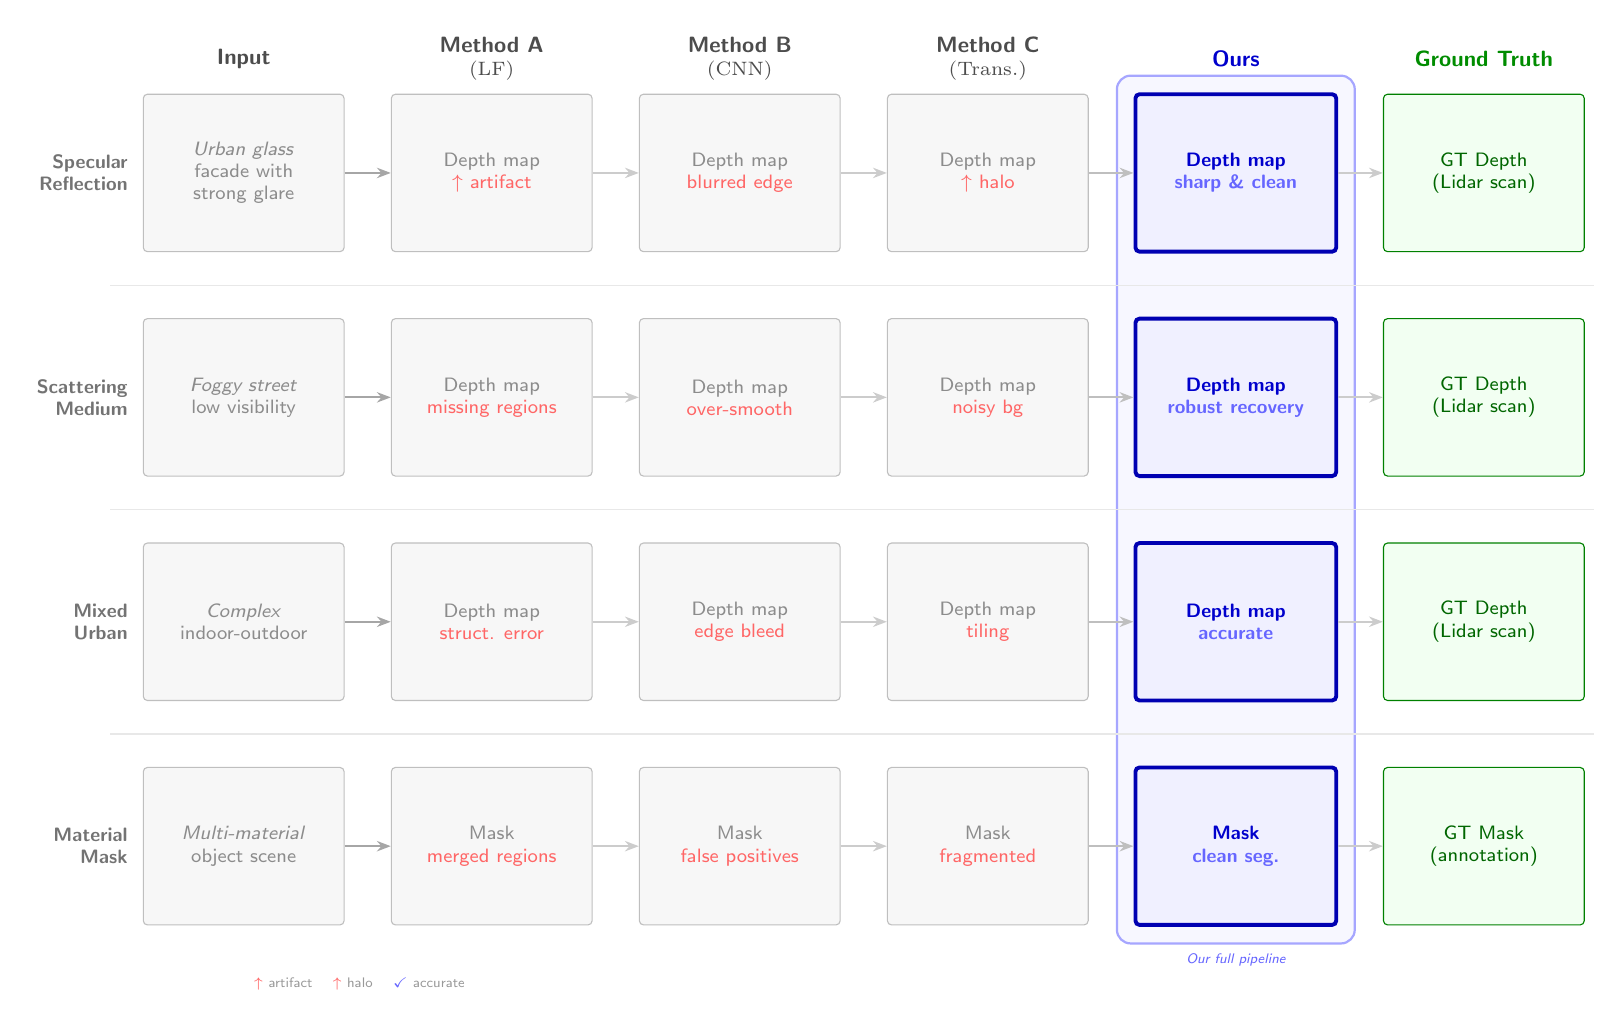
\begin{tikzpicture}[
  % --- style definitions ---
  imgbox/.style={
    draw=gray!50, rounded corners=1.5pt,
    minimum width=2.55cm, minimum height=2.0cm,
    inner sep=0pt, align=center,
    fill=gray!6, font=\sffamily\scriptsize,
    text=black!45
  },
  imgbox_ours/.style={
    imgbox,
    draw=blue!70!black, line width=1.4pt,
    fill=blue!6, font=\sffamily\scriptsize\bfseries,
    text=blue!80!black
  },
  imgbox_gt/.style={
    imgbox,
    fill=green!5, draw=green!50!black,
    text=green!40!black
  },
  colhead/.style={
    font=\sffamily\footnotesize\bfseries,
    text=black!70, align=center
  },
  scene_lbl/.style={
    font=\sffamily\scriptsize\bfseries,
    text=black!55, align=right, anchor=east
  },
  arr/.style={
    -{Stealth[length=5pt]}, thick, color=black!35
  },
  bracket/.style={
    decorate, decoration={brace, amplitude=5pt, mirror},
    thick, color=black!30
  },
]

% ============================================================
% Column positions
% ============================================================
\def\colX{0}
\def\colA{3.15}
\def\colB{6.30}
\def\colC{9.45}
\def\colO{12.60}
\def\colG{15.75}
% Row y-positions (top to bottom)
\def\rowI{0}
\def\rowII{-2.85}
\def\rowIII{-5.70}
\def\rowIV{-8.55}

% ============================================================
% Column headers
% ============================================================
\node[colhead] at (\colX, 1.45)  {Input};
\node[colhead] at (\colA, 1.45)  {Method A\\[-1pt]{\scriptsize\normalfont (LF)}};
\node[colhead] at (\colB, 1.45)  {Method B\\[-1pt]{\scriptsize\normalfont (CNN)}};
\node[colhead] at (\colC, 1.45)  {Method C\\[-1pt]{\scriptsize\normalfont (Trans.)}};
\node[colhead, text=blue!80!black] at (\colO, 1.45)  {Ours};
\node[colhead, text=green!55!black] at (\colG, 1.45)  {Ground Truth};

% ============================================================
% Row 1: Specular Reflection Scene
% ============================================================
\node[scene_lbl] at (-1.35, \rowI) {Specular\\Reflection};
\node[imgbox] (r1input) at (\colX, \rowI)
  {\textit{Urban glass}\\facade with\\strong glare};
\node[imgbox] (r1a) at (\colA, \rowI)
  {Depth map\\{\color{red!60}\scriptsize$\uparrow$ artifact}};
\node[imgbox] (r1b) at (\colB, \rowI)
  {Depth map\\{\color{red!60}\scriptsize blurred edge}};
\node[imgbox] (r1c) at (\colC, \rowI)
  {Depth map\\{\color{red!60}\scriptsize$\uparrow$ halo}};
\node[imgbox_ours] (r1o) at (\colO, \rowI)
  {Depth map\\{\color{blue!60}\scriptsize sharp \& clean}};
\node[imgbox_gt] (r1g) at (\colG, \rowI)
  {GT Depth\\(Lidar scan)};

% ============================================================
% Row 2: Scattering Medium Scene
% ============================================================
\node[scene_lbl] at (-1.35, \rowII) {Scattering\\Medium};
\node[imgbox] (r2input) at (\colX, \rowII)
  {\textit{Foggy street}\\low visibility};
\node[imgbox] (r2a) at (\colA, \rowII)
  {Depth map\\{\color{red!60}\scriptsize missing regions}};
\node[imgbox] (r2b) at (\colB, \rowII)
  {Depth map\\{\color{red!60}\scriptsize over-smooth}};
\node[imgbox] (r2c) at (\colC, \rowII)
  {Depth map\\{\color{red!60}\scriptsize noisy bg}};
\node[imgbox_ours] (r2o) at (\colO, \rowII)
  {Depth map\\{\color{blue!60}\scriptsize robust recovery}};
\node[imgbox_gt] (r2g) at (\colG, \rowII)
  {GT Depth\\(Lidar scan)};

% ============================================================
% Row 3: Mixed Urban Scene (Depth)
% ============================================================
\node[scene_lbl] at (-1.35, \rowIII) {Mixed\\Urban};
\node[imgbox] (r3input) at (\colX, \rowIII)
  {\textit{Complex}\\indoor-outdoor};
\node[imgbox] (r3a) at (\colA, \rowIII)
  {Depth map\\{\color{red!60}\scriptsize struct. error}};
\node[imgbox] (r3b) at (\colB, \rowIII)
  {Depth map\\{\color{red!60}\scriptsize edge bleed}};
\node[imgbox] (r3c) at (\colC, \rowIII)
  {Depth map\\{\color{red!60}\scriptsize tiling}};
\node[imgbox_ours] (r3o) at (\colO, \rowIII)
  {Depth map\\{\color{blue!60}\scriptsize accurate}};
\node[imgbox_gt] (r3g) at (\colG, \rowIII)
  {GT Depth\\(Lidar scan)};

% ============================================================
% Row 4: Material Mask Prediction
% ============================================================
\node[scene_lbl] at (-1.35, \rowIV) {Material\\Mask};
\node[imgbox] (r4input) at (\colX, \rowIV)
  {\textit{Multi-material}\\object scene};
\node[imgbox] (r4a) at (\colA, \rowIV)
  {Mask\\{\color{red!60}\scriptsize merged regions}};
\node[imgbox] (r4b) at (\colB, \rowIV)
  {Mask\\{\color{red!60}\scriptsize false positives}};
\node[imgbox] (r4c) at (\colC, \rowIV)
  {Mask\\{\color{red!60}\scriptsize fragmented}};
\node[imgbox_ours] (r4o) at (\colO, \rowIV)
  {Mask\\{\color{blue!60}\scriptsize clean seg.}};
\node[imgbox_gt] (r4g) at (\colG, \rowIV)
  {GT Mask\\(annotation)};

% ============================================================
% Flow arrows (input -> methods -> ours -> GT)
% ============================================================
\foreach \r in {1,2,3,4} {
  % input to Method A
  \draw[arr] (r\r input.east) -- (r\r a.west);
  % Method A to B
  \draw[arr, color=black!20] (r\r a.east) -- (r\r b.west);
  % Method B to C
  \draw[arr, color=black!20] (r\r b.east) -- (r\r c.west);
  % Method C to Ours
  \draw[arr, color=black!25] (r\r c.east) -- (r\r o.west);
  % Ours to GT
  \draw[arr, color=black!20] (r\r o.east) -- (r\r g.west);
}

% ============================================================
% Highlight boxes: "Ours" column
% ============================================================
\begin{scope}[on background layer]
  \node[draw=blue!35, fill=blue!3, rounded corners=5pt,
        inner xsep=6pt, inner ysep=6pt, line width=0.8pt,
        fit=(r1o)(r2o)(r3o)(r4o)] (oursbox) {};
\end{scope}

% "Best" annotation
\node[font=\sffamily\tiny\itshape, text=blue!60,
      anchor=north] at (oursbox.south)
  {Our full pipeline};

% ============================================================
% Error legend (small)
% ============================================================
\node[anchor=north west, font=\sffamily\tiny, text=black!40,
      align=left]
  at (\colX, \rowIV - 1.55)
  {{\color{red!60}$\uparrow$} artifact \quad
   {\color{red!60}$\uparrow$} halo \quad
   {\color{blue!60}$\checkmark$} accurate};

% ============================================================
% Scene separator lines
% ============================================================
\foreach \yy in {-1.425, -4.275, -7.125} {
  \draw[gray!18, line width=0.4pt] (-1.7, \yy) -- (\colG+1.4, \yy);
}

\end{tikzpicture}
\end{document}